\section{引言}
工欲善其事,必先利其器。优秀的工具辅助,通常能使工作效率大幅度提升。
而我们今天所要介绍的Tbrowser Remote DevTools(Tbrowser远程页面调试工具)就是这样的利器。
它能使TV上页面调试工作拥有和PC上几乎一样的体验。
话不多说,让我们尽快开始Tbrowser Remote DevTools学习之旅吧。

\section{打开Tbrowser Remote DevTools}
为了保证浏览器性能,Tbrowser Remote DevTools是默认关闭的。
不过,只需要简单的操作就可以打开此功能。
我们提供两种方法打开Tbrowser调试功能:

\begin{itemize}
  \item \textbf{通过tcli命令打开}\\
  需要执行的命令是:/tvos/bin/tcli tbrw2.enabledevtools.pid\\
  pid是浏览器的进程号,可以通过 /tvos/bin/tcli help | grep tbrw2 命令查看。\\
  这种打开方式不需要重启TV,直接可以使用。但重启之后失效,还需再次执行命令。
  \begin{figure}[H] 
  \centering 
  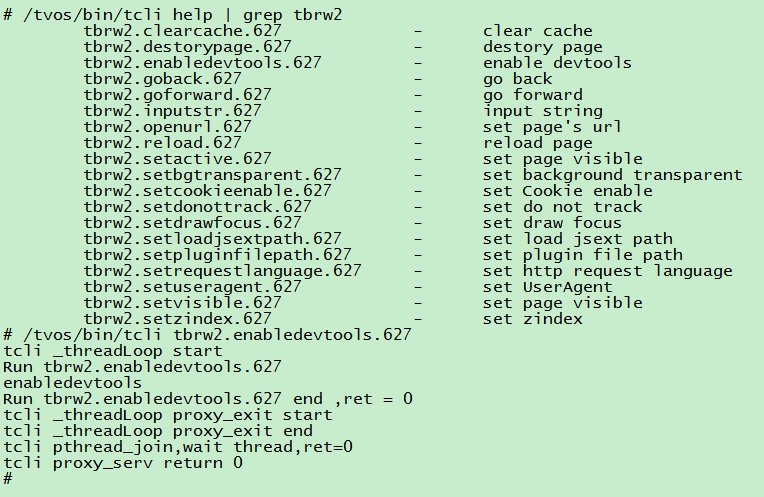
\includegraphics[width=0.9\textwidth]{image/devtools_study/tcli_command.PNG} 
  \caption{通过tcli打开过程} \label{fig:tcli_command} 
  \end{figure}
  
  \item \textbf{通过添加启动参数}\\
  需要添加的参数是:--remote-debugging-port=9222\\
  修改启动Tbrowser的run\_weblauncher\_server.sh脚本,添加上述的启动参数,重启TV即可。
  此种打开方式会一直打开Tbrowser Remote DevTools,重启依然有效,所以请不要再SQA的机器上这样修改。
\end{itemize}

Tbrowser Remote DevTools功能打开后,Tbrowser会监听指定的端口,创建一个http服务,供PC端访问。
可以通过 netstat -anp 命令查看系统的端口使用情况。
如果Tbrowser Remote DevTools功能开启,你将看到图\ref{fig:netstat_command}中的信息。
其中显示的IP是你机器的IP地址。如果使用tcli打开,端口默认是9222;如果添加了启动参数,那么端口就是参数中指定的端口号。
\begin{figure}[H] 
\centering 
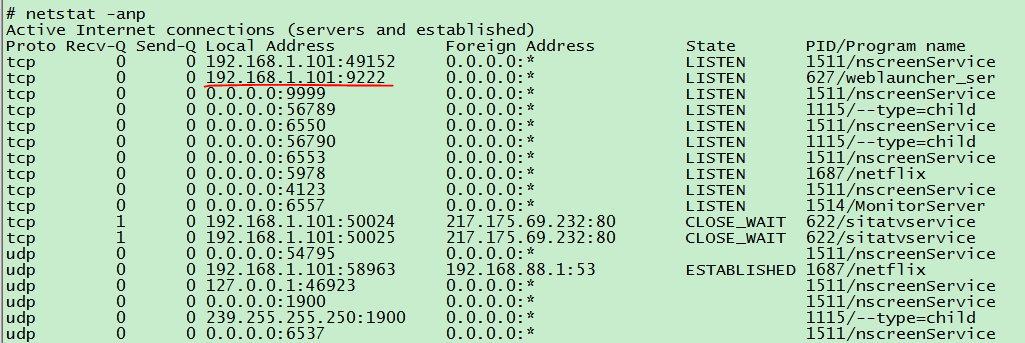
\includegraphics[width=0.9\textwidth]{image/devtools_study/netstat.PNG} 
\caption{netstat -anp命令输出结果} \label{fig:netstat_command} 
\end{figure}

到这里就非常接近成功了,后续要做的事情就是将PC连接到TV所在的网络(必须是直接连接,使用代理是不行的)。
打开PC上的Chrome浏览器,输出Tbrowser监听的地址,如上图应该是http://192.168.1.101:9222 。
如果一切顺利,你将看到图\ref{fig:home_page}中显示的内容。
其中BBC iPlayer、index.html、livetv、systemUi为打开的链接title。
如果此时浏览器没有打开任何页面,将没有任何链接。
\begin{figure}[H] 
\centering 
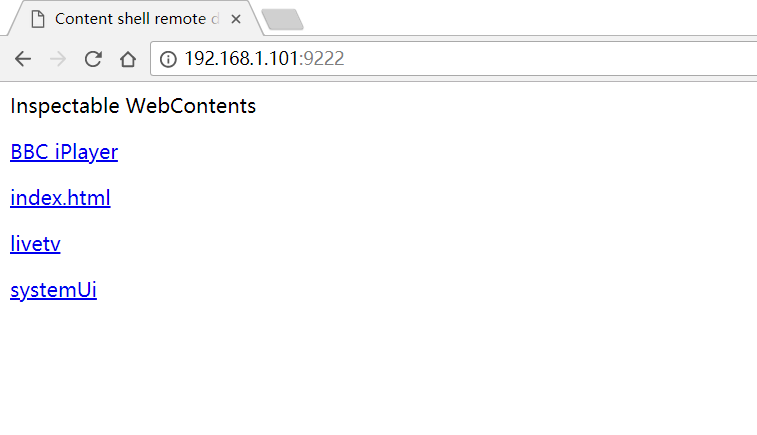
\includegraphics[width=0.9\textwidth]{image/devtools_study/home.PNG} 
\caption{Tbrowser Remote DevTools首页} \label{fig:home_page} 
\end{figure}

你可以点击其中的一个链接,进入调试页面,例如我打开BBC iPlayer链接,显示的效果如图\ref{fig:debug_page}所示。
至此,Tbrowser Remote DevTools功能已经准备妥当,下一步就可以进行页面调试了。
\begin{figure}[H] 
\centering 
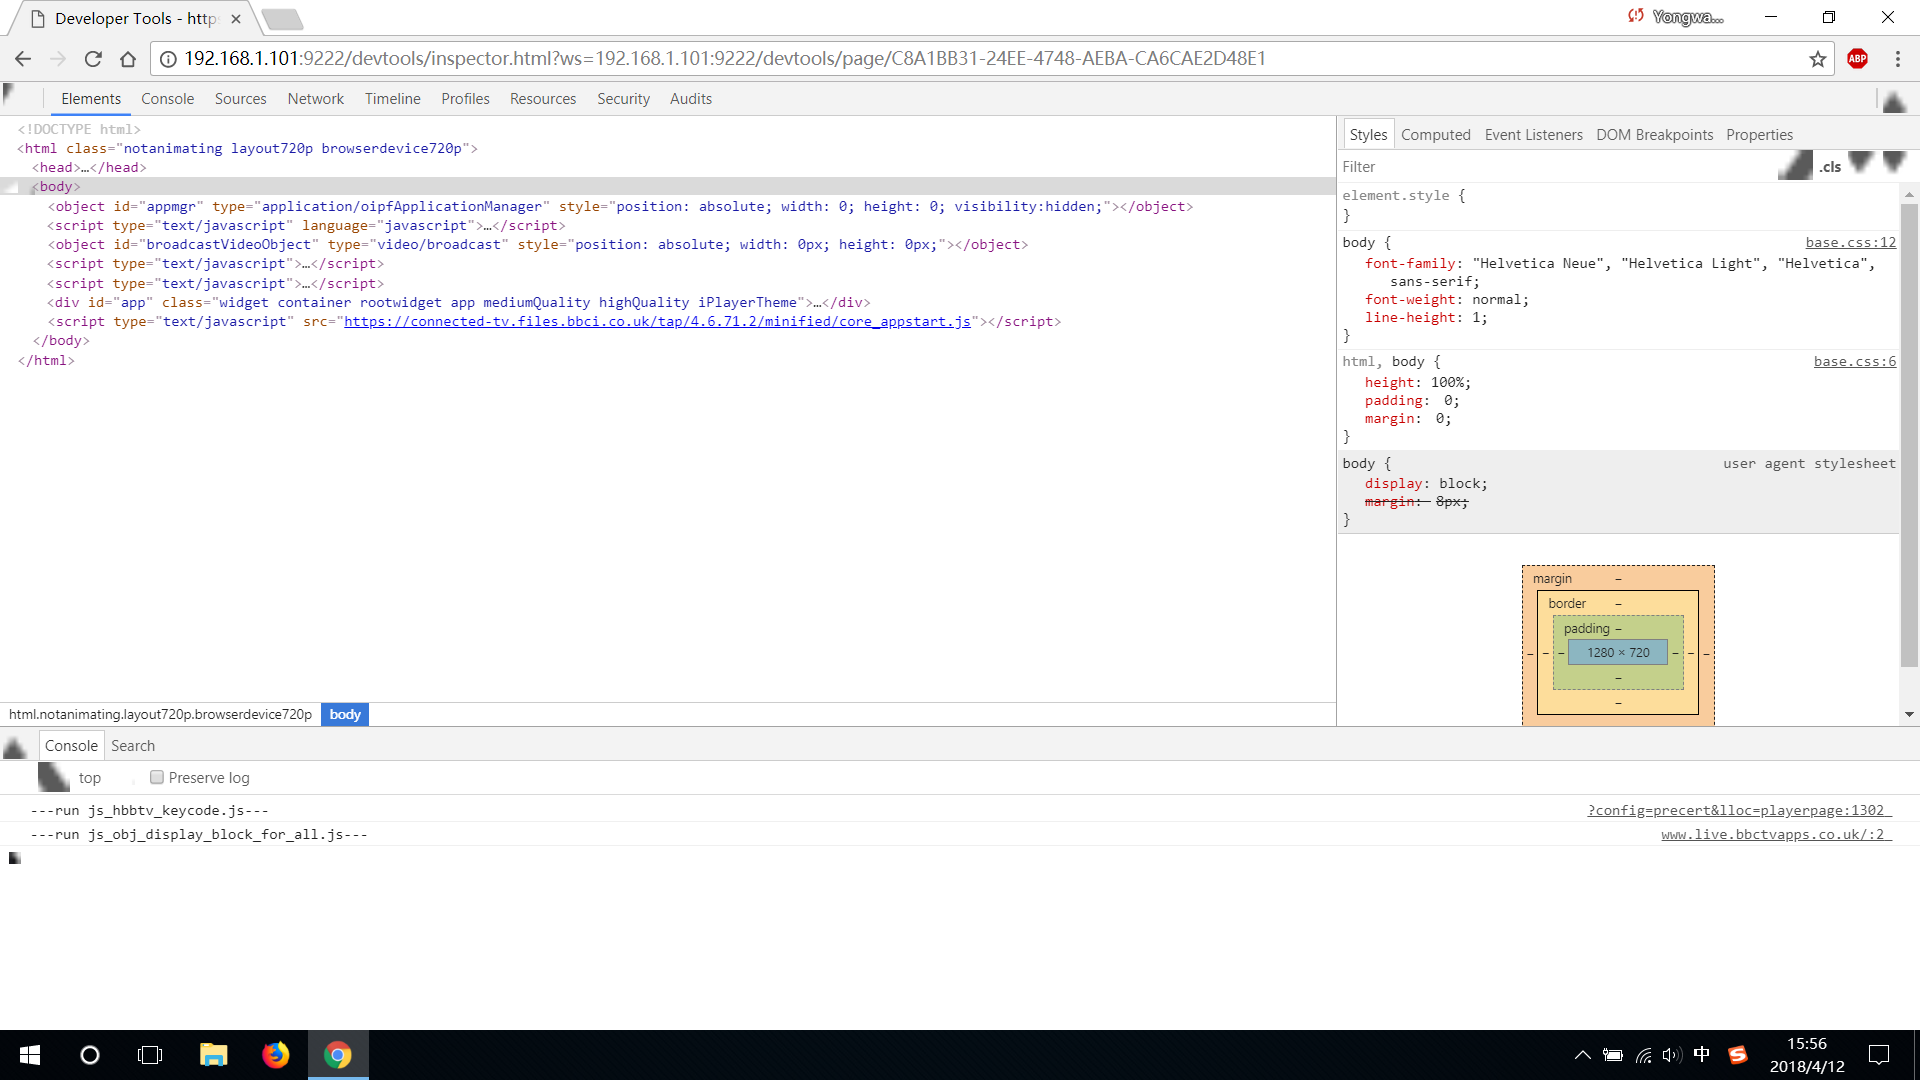
\includegraphics[width=0.9\textwidth]{image/devtools_study/debug_page.png} 
\caption{Tbrowser Remote DevTools调试页面} \label{fig:debug_page} 
\end{figure}

\section{使用Tbrowser Remote DevTools}
目前的Tbrowser2.0是基于Chromium49开发的,所以这里看到的调试页面是Chromium49版的调试页面。
有些功能和PC上的开发者工具不同,但大多数常用的功能还是一致的。
这里我们按照模块来研究一下Tbrowser Remote DevTools的具体使用情况。

\subsection{Elements模块}
此模块功能和最新的Chrome DevTools几乎没有区别,对于页面开发者来说这个模块的功能也应该非常熟悉。
此模块主要用于调试页面样式,定位页面元素监听的消息等功能。

\subsection{Console模块}
\subsection{Sources模块}
\subsection{Network模块}
\subsection{Timeline模块}
\subsection{Profiles模块}
\subsection{Resourcess模块}
\subsection{Security模块}
\subsection{Audits模块}